\subsection{Architektur und Aufbau}

Die App \textit{Locals} ist eine mobile Anwendung, die Nutzer:innen dabei
unterstützt, lokale Events zu entdecken, zu erstellen und zu verwalten. Sie
richtet sich insbesondere an ein junges, urbanes Publikum und fördert soziale
Interaktionen im Kontext gemeinsamer Veranstaltungen.

% \begin{figure}[htbp]
%     \centering
%     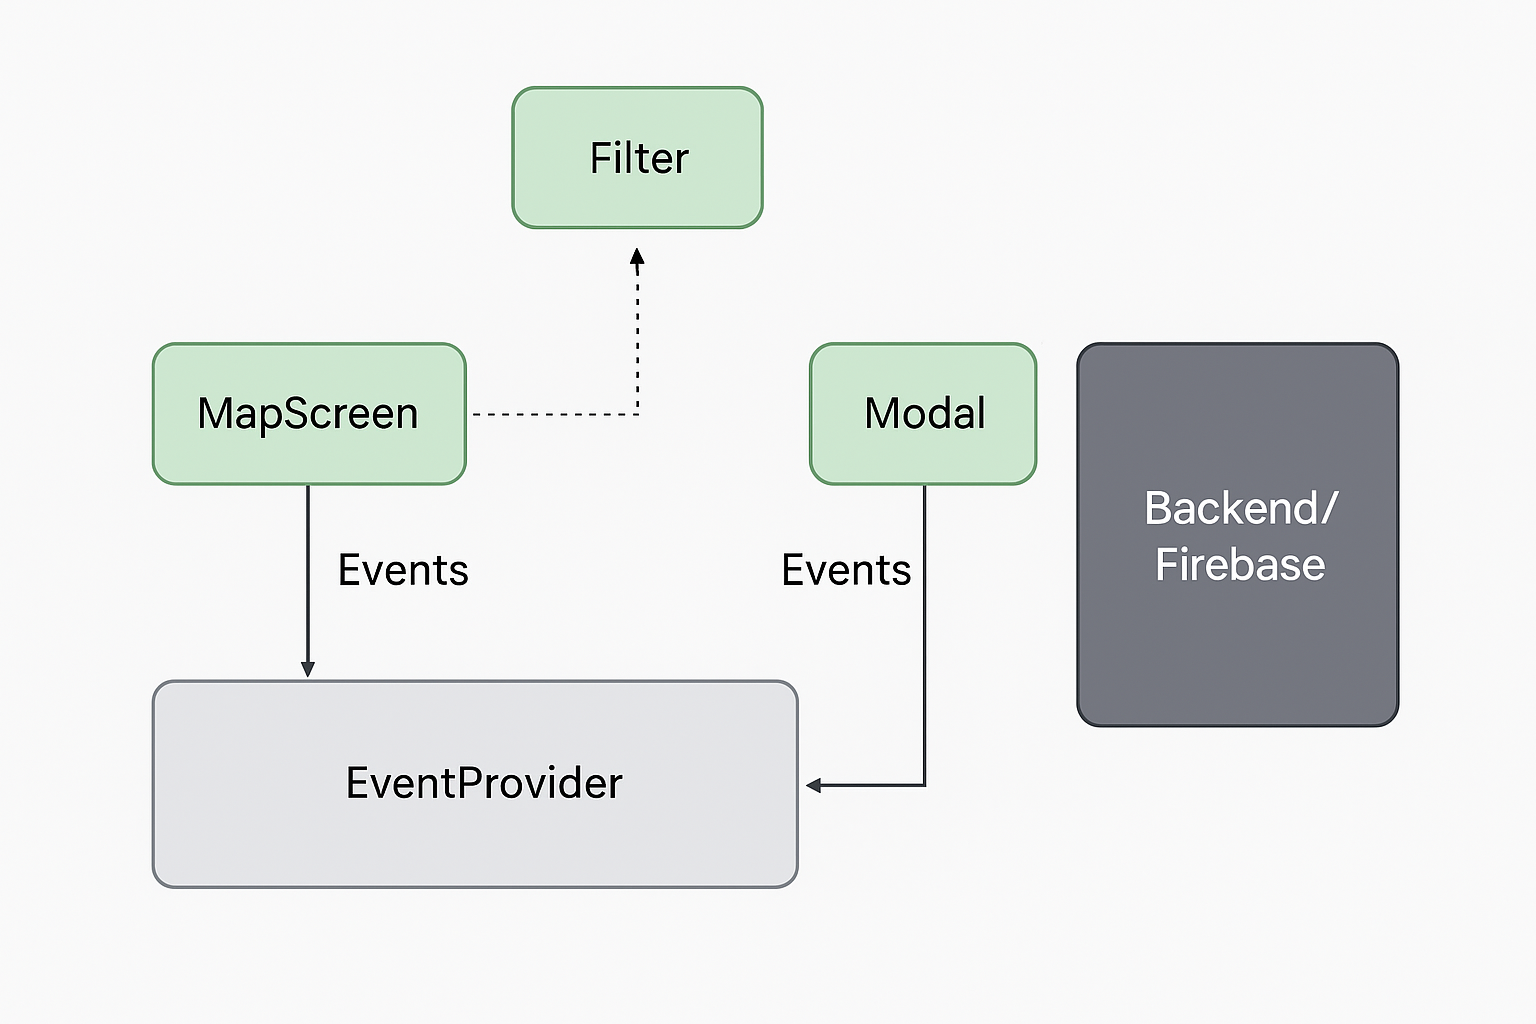
\includegraphics[width=0.95\textwidth]{images/architekturdiagramm_locals.png}
%     \caption{Architektur der App „Locals“: Darstellung der Hauptkomponenten (MapScreen, Filter, Modal, EventProvider, Backend/Firebase) und deren Datenflüsse.}
%     \label{fig:architektur-locals}
% \end{figure}

\subsubsection{Technologischer Stack und Architektur}

Der technologische Stack von \textit{Locals} wurde gezielt so ausgewählt, dass
eine moderne, plattformübergreifende Entwicklung und eine reibungslose User
Experience möglich sind:
\begin{itemize}
    \item \textbf{Frontend:} Entwicklung mit React Native, TypeScript und Expo für eine performante Bereitstellung auf iOS und Android.
    \item \textbf{Backend:} Verwendung von Firebase zur Authentifizierung, Datenhaltung und Synchronisation.
    \item \textbf{Navigation:} Einsatz von \texttt{@react-navigation/native} und \texttt{expo-router} für ein modernes, tab-basiertes Navigationskonzept.
    \item \textbf{State-Management:} Implementierung eigener Context-Provider (\texttt{AuthProvider}, \texttt{EventsProvider}) für Authentifizierungs- und Eventdaten.
    \item \textbf{UI-Komponenten:} Nutzung von \texttt{@expo/vector-icons} und \texttt{lucide-react-native} für ein ansprechendes und konsistentes User Interface.
    \item \textbf{Maps \& Location:} Integration von \texttt{react-native-maps} und \texttt{expo-location} für eine interaktive Kartenansicht, die sowohl den Nutzerstandort als auch Events auf einer Karte visualisiert.
\end{itemize}

Die App ist modular aufgebaut und besteht aus drei zentralen Bereichen:
\begin{itemize}
    \item \textbf{Explore-Screen:} Zeigt einen Event-Feed, der sich nach Interessen und aktuellem Standort richtet.
    \item \textbf{Map-Screen:} Bietet eine interaktive Kartenansicht mit Event-Markern und Filterfunktion.
    \item \textbf{Profil-Screen:} Ermöglicht die Übersicht und Verwaltung eigener Events und Profildaten.
\end{itemize}

Während Explore- und Profil-Screen bereits Grundfunktionen aufweisen, wird der
Map-Screen im Rahmen dieser Arbeit als prototypisches Demonstrationsbeispiel
gezielt entwickelt und evaluiert. Die praktische Realisierung dieses Features
erfolgt unter Einsatz generativer KI-Tools und steht im Mittelpunkt der
folgenden Kapitel.

\subsubsection{Struktur der Haupteinstiegskomponente (\texttt{RootLayout})}

Die zentrale Einstiegskomponente der App ist das \texttt{RootLayout}. Diese
übernimmt das Laden benutzerdefinierter Fonts, die Einbindung von
Authentifizierungs- und Events-Kontexten sowie eine durchgängige Nutzerführung
nach dem Login. Die Navigation wird dabei strikt vom Authentifizierungsstatus
gesteuert, sodass nicht eingeloggte Nutzer:innen automatisch zur Login-Ansicht
weitergeleitet werden. Für die technische Umsetzung werden Hooks wie
\texttt{useAuth}, \texttt{useSegments} und \texttt{useRouter} eingesetzt.

\subsection{Bestehende Funktionalitäten}

Bereits implementierte Kernfunktionen von \textit{Locals} sind:
\begin{itemize}
    \item \textbf{Benutzerauthentifizierung:} Sichere Registrierung und Anmeldung über Firebase Authentication.
    \item \textbf{Profilverwaltung:} Verwaltung persönlicher Daten sowie Übersicht über besuchte und selbst erstellte Events.
    \item \textbf{Eventverwaltung:} Anlegen, Bearbeiten und Löschen von Events.
    \item \textbf{Tab-Navigation:} Ermöglicht den nahtlosen Wechsel zwischen den drei Hauptbereichen „Explore“, „Map“ und „Profil“.
    \item \textbf{Responsives Design:} Konsistente Darstellung auf verschiedenen Endgeräten durch Nutzung von \texttt{react-native-safe-area-context} und Expo UI-Komponenten.
\end{itemize}

Der Map-Screen ist als zentrales, innovatives Feature der App konzipiert. Die
Implementierung und Weiterentwicklung dieses Moduls wird im weiteren Verlauf
dieser Arbeit als praktisches Beispiel für den Einsatz generativer KI in der
Softwareentwicklung detailliert analysiert.
